% Automatically generated by go_latex.py
%
\renewcommand{\one}{real_wall-plaster-white}
\renewcommand{\two}{real_plastic-red-carton}
\renewcommand{\thr}{real_leather-blue}
\renewcommand{\fou}{real_bathroomtile2}
\renewcommand{\fiv}{real_wood-walnut}
\renewcommand{\six}{real_wood-tile}
\renewcommand{\sev}{real_book1}
\renewcommand{\eit}{real_book2}
\renewcommand{\nin}{real_giftbag1}
\renewcommand{\ten}{real_cards-red}

\setlength{\resLen}{.48in}
\begin{figure*}[htbp]
    \centering
    \small
    \addtolength{\tabcolsep}{-4pt}
    \begin{tabular}{rlrccc@{\hspace{2\tabcolsep}}lrccc}
        & \multicolumn{2}{c}{\textbf{SVBRDF maps}} & \textbf{Opt.} & \multicolumn{2}{c}{\textbf{Novel views}}
        & \multicolumn{2}{c}{\textbf{SVBRDF maps}} & \textbf{Opt.} & \multicolumn{2}{c}{\textbf{Novel views}}
        \\[1pt]
        &
        \raisebox{3pt}{\textit{~~wall-plaster-white}} & \raisebox{0.40\resLen}{\rotatebox[origin=c]{90}{\scriptsize GT}}&
        \includegraphics[height=\resLen]{results/main/\one/ref/00.jpg} &
        \includegraphics[height=\resLen]{results/main/\one/ref/07.jpg} &
        \includegraphics[height=\resLen]{results/main/\one/ref/08.jpg} &
        \raisebox{3pt}{\textit{~~plastic-red-carton}} & \raisebox{0.40\resLen}{\rotatebox[origin=c]{90}{\scriptsize GT}}&
        \includegraphics[height=\resLen]{results/main/\two/ref/00.jpg} &
        \includegraphics[height=\resLen]{results/main/\two/ref/07.jpg} &
        \includegraphics[height=\resLen]{results/main/\two/ref/08.jpg}
        \\
        \raisebox{0.40\resLen}{\rotatebox[origin=c]{90}{\scriptsize Ours}} &
        \multicolumn{2}{c}{\includegraphics[height=\resLen]{results/main/\one/ours+/tex.jpg}} &
        \includegraphics[height=\resLen]{results/main/\one/ours+/00.jpg} &
        \includegraphics[height=\resLen]{results/main/\one/ours+/07.jpg} &
        \includegraphics[height=\resLen]{results/main/\one/ours+/08.jpg} &
        \multicolumn{2}{c}{\includegraphics[height=\resLen]{results/main/\two/ours+/tex.jpg}} &
        \includegraphics[height=\resLen]{results/main/\two/ours+/00.jpg} &
        \includegraphics[height=\resLen]{results/main/\two/ours+/07.jpg} &
        \includegraphics[height=\resLen]{results/main/\two/ours+/08.jpg}
        \\
        \raisebox{0.40\resLen}{\rotatebox[origin=c]{90}{\scriptsize [Gao19]+}} &
        \multicolumn{2}{c}{\includegraphics[height=\resLen]{results/main/\one/msra+_egsr/tex.jpg}} &
        \includegraphics[height=\resLen]{results/main/\one/msra+_egsr/00.jpg} &
        \includegraphics[height=\resLen]{results/main/\one/msra+_egsr/07.jpg} &
        \includegraphics[height=\resLen]{results/main/\one/msra+_egsr/08.jpg} &
        \multicolumn{2}{c}{\includegraphics[height=\resLen]{results/main/\two/msra+_egsr/tex.jpg}} &
        \includegraphics[height=\resLen]{results/main/\two/msra+_egsr/00.jpg} &
        \includegraphics[height=\resLen]{results/main/\two/msra+_egsr/07.jpg} &
        \includegraphics[height=\resLen]{results/main/\two/msra+_egsr/08.jpg}
        \\[1pt]
        &
        \raisebox{3pt}{\textit{~~leather-blue}} & \raisebox{0.40\resLen}{\rotatebox[origin=c]{90}{\scriptsize GT}}&
        \includegraphics[height=\resLen]{results/main/\thr/ref/00.jpg} &
        \includegraphics[height=\resLen]{results/main/\thr/ref/07.jpg} &
        \includegraphics[height=\resLen]{results/main/\thr/ref/08.jpg} &
        \raisebox{3pt}{\textit{~~bathroomtile2}} & \raisebox{0.40\resLen}{\rotatebox[origin=c]{90}{\scriptsize GT}}&
        \includegraphics[height=\resLen]{results/main/\fou/ref/00.jpg} &
        \includegraphics[height=\resLen]{results/main/\fou/ref/07.jpg} &
        \includegraphics[height=\resLen]{results/main/\fou/ref/08.jpg}
        \\
        \raisebox{0.40\resLen}{\rotatebox[origin=c]{90}{\scriptsize Ours}} &
        \multicolumn{2}{c}{\includegraphics[height=\resLen]{results/main/\thr/ours+/tex.jpg}} &
        \includegraphics[height=\resLen]{results/main/\thr/ours+/00.jpg} &
        \includegraphics[height=\resLen]{results/main/\thr/ours+/07.jpg} &
        \includegraphics[height=\resLen]{results/main/\thr/ours+/08.jpg} &
        \multicolumn{2}{c}{\includegraphics[height=\resLen]{results/main/\fou/ours+/tex.jpg}} &
        \includegraphics[height=\resLen]{results/main/\fou/ours+/00.jpg} &
        \includegraphics[height=\resLen]{results/main/\fou/ours+/07.jpg} &
        \includegraphics[height=\resLen]{results/main/\fou/ours+/08.jpg}
        \\
        \raisebox{0.40\resLen}{\rotatebox[origin=c]{90}{\scriptsize [Gao19]+}} &
        \multicolumn{2}{c}{\includegraphics[height=\resLen]{results/main/\thr/msra+_egsr/tex.jpg}} &
        \includegraphics[height=\resLen]{results/main/\thr/msra+_egsr/00.jpg} &
        \includegraphics[height=\resLen]{results/main/\thr/msra+_egsr/07.jpg} &
        \includegraphics[height=\resLen]{results/main/\thr/msra+_egsr/08.jpg} &
        \multicolumn{2}{c}{\includegraphics[height=\resLen]{results/main/\fou/msra+_egsr/tex.jpg}} &
        \includegraphics[height=\resLen]{results/main/\fou/msra+_egsr/00.jpg} &
        \includegraphics[height=\resLen]{results/main/\fou/msra+_egsr/07.jpg} &
        \includegraphics[height=\resLen]{results/main/\fou/msra+_egsr/08.jpg}
        \\[1pt]
        &
        \raisebox{3pt}{\textit{~~wood-walnut}} & \raisebox{0.40\resLen}{\rotatebox[origin=c]{90}{\scriptsize GT}}&
        \includegraphics[height=\resLen]{results/main/\fiv/ref/00.jpg} &
        \includegraphics[height=\resLen]{results/main/\fiv/ref/07.jpg} &
        \includegraphics[height=\resLen]{results/main/\fiv/ref/08.jpg} &
        \raisebox{3pt}{\textit{~~wood-tile}} & \raisebox{0.40\resLen}{\rotatebox[origin=c]{90}{\scriptsize GT}}&
        \includegraphics[height=\resLen]{results/main/\six/ref/00.jpg} &
        \includegraphics[height=\resLen]{results/main/\six/ref/07.jpg} &
        \includegraphics[height=\resLen]{results/main/\six/ref/08.jpg}
        \\
        \raisebox{0.40\resLen}{\rotatebox[origin=c]{90}{\scriptsize Ours}} &
        \multicolumn{2}{c}{\includegraphics[height=\resLen]{results/main/\fiv/ours+/tex.jpg}} &
        \includegraphics[height=\resLen]{results/main/\fiv/ours+/00.jpg} &
        \includegraphics[height=\resLen]{results/main/\fiv/ours+/07.jpg} &
        \includegraphics[height=\resLen]{results/main/\fiv/ours+/08.jpg} &
        \multicolumn{2}{c}{\includegraphics[height=\resLen]{results/main/\six/ours+/tex.jpg}} &
        \includegraphics[height=\resLen]{results/main/\six/ours+/00.jpg} &
        \includegraphics[height=\resLen]{results/main/\six/ours+/07.jpg} &
        \includegraphics[height=\resLen]{results/main/\six/ours+/08.jpg}
        \\
        \raisebox{0.40\resLen}{\rotatebox[origin=c]{90}{\scriptsize [Gao19]+}} &
        \multicolumn{2}{c}{\includegraphics[height=\resLen]{results/main/\fiv/msra+_egsr/tex.jpg}} &
        \includegraphics[height=\resLen]{results/main/\fiv/msra+_egsr/00.jpg} &
        \includegraphics[height=\resLen]{results/main/\fiv/msra+_egsr/07.jpg} &
        \includegraphics[height=\resLen]{results/main/\fiv/msra+_egsr/08.jpg} &
        \multicolumn{2}{c}{\includegraphics[height=\resLen]{results/main/\six/msra+_egsr/tex.jpg}} &
        \includegraphics[height=\resLen]{results/main/\six/msra+_egsr/00.jpg} &
        \includegraphics[height=\resLen]{results/main/\six/msra+_egsr/07.jpg} &
        \includegraphics[height=\resLen]{results/main/\six/msra+_egsr/08.jpg}
        \\[1pt]
        &
        \raisebox{3pt}{\textit{~~book1}} & \raisebox{0.40\resLen}{\rotatebox[origin=c]{90}{\scriptsize GT}}&
        \includegraphics[height=\resLen]{results/main/\sev/ref/00.jpg} &
        \includegraphics[height=\resLen]{results/main/\sev/ref/07.jpg} &
        \includegraphics[height=\resLen]{results/main/\sev/ref/08.jpg} &
        \raisebox{3pt}{\textit{~~book2}} & \raisebox{0.40\resLen}{\rotatebox[origin=c]{90}{\scriptsize GT}}&
        \includegraphics[height=\resLen]{results/main/\eit/ref/00.jpg} &
        \includegraphics[height=\resLen]{results/main/\eit/ref/07.jpg} &
        \includegraphics[height=\resLen]{results/main/\eit/ref/08.jpg}
        \\
        \raisebox{0.40\resLen}{\rotatebox[origin=c]{90}{\scriptsize Ours}} &
        \multicolumn{2}{c}{\includegraphics[height=\resLen]{results/main/\sev/ours+/tex.jpg}} &
        \includegraphics[height=\resLen]{results/main/\sev/ours+/00.jpg} &
        \includegraphics[height=\resLen]{results/main/\sev/ours+/07.jpg} &
        \includegraphics[height=\resLen]{results/main/\sev/ours+/08.jpg} &
        \multicolumn{2}{c}{\includegraphics[height=\resLen]{results/main/\eit/ours+/tex.jpg}} &
        \includegraphics[height=\resLen]{results/main/\eit/ours+/00.jpg} &
        \includegraphics[height=\resLen]{results/main/\eit/ours+/07.jpg} &
        \includegraphics[height=\resLen]{results/main/\eit/ours+/08.jpg}
        \\
        \raisebox{0.40\resLen}{\rotatebox[origin=c]{90}{\scriptsize [Gao19]+}} &
        \multicolumn{2}{c}{\includegraphics[height=\resLen]{results/main/\sev/msra+_egsr/tex.jpg}} &
        \includegraphics[height=\resLen]{results/main/\sev/msra+_egsr/00.jpg} &
        \includegraphics[height=\resLen]{results/main/\sev/msra+_egsr/07.jpg} &
        \includegraphics[height=\resLen]{results/main/\sev/msra+_egsr/08.jpg} &
        \multicolumn{2}{c}{\includegraphics[height=\resLen]{results/main/\eit/msra+_egsr/tex.jpg}} &
        \includegraphics[height=\resLen]{results/main/\eit/msra+_egsr/00.jpg} &
        \includegraphics[height=\resLen]{results/main/\eit/msra+_egsr/07.jpg} &
        \includegraphics[height=\resLen]{results/main/\eit/msra+_egsr/08.jpg}
        \\[1pt]
        &
        \raisebox{3pt}{\textit{~~giftbag1}} & \raisebox{0.40\resLen}{\rotatebox[origin=c]{90}{\scriptsize GT}}&
        \includegraphics[height=\resLen]{results/main/\nin/ref/00.jpg} &
        \includegraphics[height=\resLen]{results/main/\nin/ref/07.jpg} &
        \includegraphics[height=\resLen]{results/main/\nin/ref/08.jpg} &
        \raisebox{3pt}{\textit{~~cards-red}} & \raisebox{0.40\resLen}{\rotatebox[origin=c]{90}{\scriptsize GT}}&
        \includegraphics[height=\resLen]{results/main/\ten/ref/00.jpg} &
        \includegraphics[height=\resLen]{results/main/\ten/ref/07.jpg} &
        \includegraphics[height=\resLen]{results/main/\ten/ref/08.jpg}
        \\
        \raisebox{0.40\resLen}{\rotatebox[origin=c]{90}{\scriptsize Ours}} &
        \multicolumn{2}{c}{\includegraphics[height=\resLen]{results/main/\nin/ours+/tex.jpg}} &
        \includegraphics[height=\resLen]{results/main/\nin/ours+/00.jpg} &
        \includegraphics[height=\resLen]{results/main/\nin/ours+/07.jpg} &
        \includegraphics[height=\resLen]{results/main/\nin/ours+/08.jpg} &
        \multicolumn{2}{c}{\includegraphics[height=\resLen]{results/main/\ten/ours+/tex.jpg}} &
        \includegraphics[height=\resLen]{results/main/\ten/ours+/00.jpg} &
        \includegraphics[height=\resLen]{results/main/\ten/ours+/07.jpg} &
        \includegraphics[height=\resLen]{results/main/\ten/ours+/08.jpg}
        \\
        \raisebox{0.40\resLen}{\rotatebox[origin=c]{90}{\scriptsize [Gao19]+}} &
        \multicolumn{2}{c}{\includegraphics[height=\resLen]{results/main/\nin/msra+_egsr/tex.jpg}} &
        \includegraphics[height=\resLen]{results/main/\nin/msra+_egsr/00.jpg} &
        \includegraphics[height=\resLen]{results/main/\nin/msra+_egsr/07.jpg} &
        \includegraphics[height=\resLen]{results/main/\nin/msra+_egsr/08.jpg} &
        \multicolumn{2}{c}{\includegraphics[height=\resLen]{results/main/\ten/msra+_egsr/tex.jpg}} &
        \includegraphics[height=\resLen]{results/main/\ten/msra+_egsr/00.jpg} &
        \includegraphics[height=\resLen]{results/main/\ten/msra+_egsr/07.jpg} &
        \includegraphics[height=\resLen]{results/main/\ten/msra+_egsr/08.jpg}
    \end{tabular}
    \caption{\label{fig:real}
        \textbf{SVBRDF reconstruction on real data.}
        We reconstruct SVBRDF maps from 7 inputs, and compare the resulting maps and images rendered under 2 novel views.
        Gao's method~\shortcite{Gao2019} initialized with Deschaintre's~\shortcite{Deschaintre2019} direct predictions (denoted as ``[Gao19]+'') tends to have complex reflectance burnt into the specular albedo map, leading to inaccurate predictions under novel views.
        Our method with simple initializations, in contrast, is less prone to such burn-ins and generally produces more accurate renderings under novel views.
        Please refer to Table~\ref{tab:main} for more information on the quality of these renderings.
    }
\end{figure*}
